\documentclass[11pt]{article}
\usepackage[latin1]{inputenc}
\usepackage{tikz}
\usepackage{caption}
\usepackage[margin=0.25in]{geometry}
\usetikzlibrary{shapes,arrows}
\newcommand*{\h}{\hspace{5pt}}% for indentation
\newcommand*{\hh}{\h\h}% double indentation
\begin{document}
\begin{center}
  \captionof{figure}{Flowchart of Calcium Hydroxide and Hydrochloric acid Titration}
  \footnotesize
  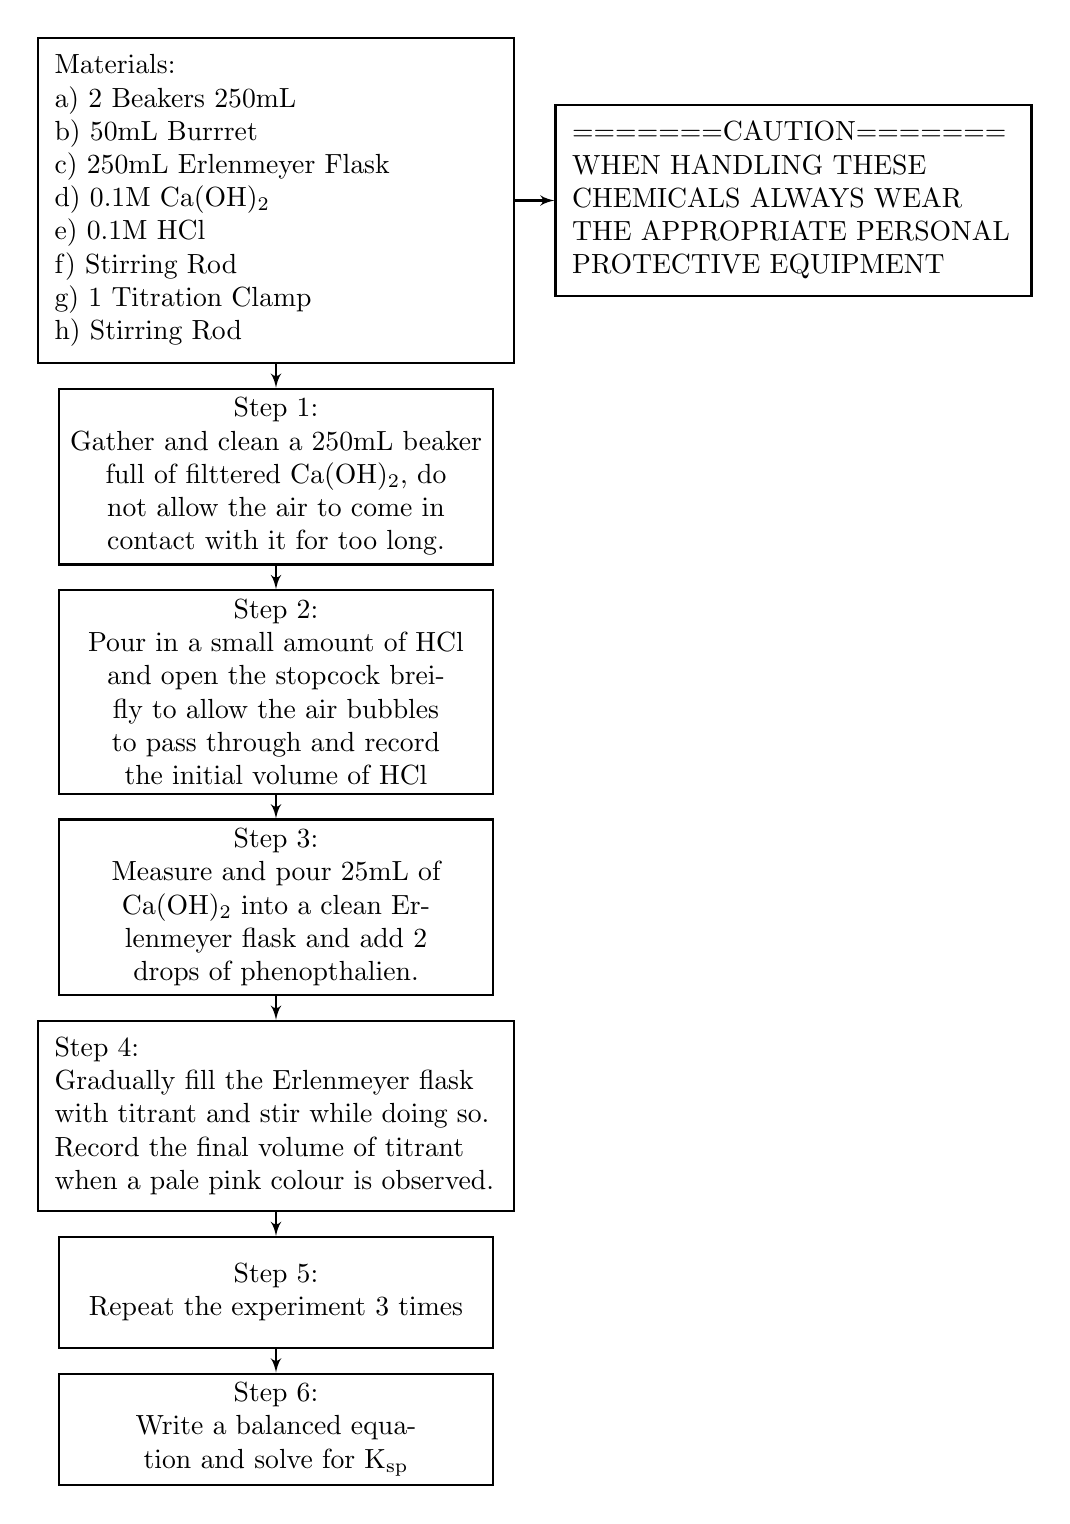
\begin{tikzpicture}[auto,
    %decision/.style={diamond, draw=black, thick, fill=white,
    %text width=8em, text badly centered,
    %inner sep=1pt, font=\sffamily\small},
    block_center/.style ={rectangle, draw=black, thick, fill=white, text width=15em, text centered,
      minimum height=4em},
    block_left/.style ={rectangle, draw=black, thick, fill=white,
      text width=16em, text ragged, minimum height=4em, inner sep=6pt},
    block_noborder/.style ={rectangle, draw=none, thick, fill=none,
      text width=18em, text centered, minimum height=1em},
    block_assign/.style ={rectangle, draw=black, thick, fill=white,
      text width=18em, text ragged, minimum height=3em, inner sep=6pt},
    block_lost/.style ={rectangle, draw=black, thick, fill=white,
      text width=16em, text ragged, minimum height=3em, inner sep=6pt},
      line/.style ={draw, thick, -latex', shorten >=0pt}]
    % outlining the flowchart using the PGF/TikZ matrix funtion
    \matrix [column sep=5mm,row sep=3mm] {
      % enrollment - row 1
		\node [block_left] (materials) {
		Materials: \\
        	a) 2 Beakers 250mL\\
        	b) 50mL Burrret\\
        	c) 250mL Erlenmeyer Flask\\
	        d) 0.1M Ca(OH)\textsubscript{2}\\
        	e) 0.1M HCl \\
        	f) Stirring Rod\\
        	g) 1 Titration Clamp\\
        	h) Stirring Rod\\};
		& \node [block_left] (caution) {
		=======CAUTION======= \\
        	WHEN HANDLING THESE CHEMICALS ALWAYS WEAR THE APPROPRIATE PERSONAL PROTECTIVE EQUIPMENT}; \\
      % enrollment - row 2
		\node [block_center] (step1) {
		Step 1: \\
		Gather and clean a 250mL beaker full of filttered Ca(OH)\textsubscript{2}, do not allow the air to come in contact with it for too long.};\\
		\node [block_center] (step2) {
		Step 2: \\
		Pour in a small amount of HCl and open the stopcock breifly to allow the air bubbles to pass through and record the initial volume of HCl};\\
		\node [block_center] (step3) {
		Step 3: \\
		Measure and pour 25mL of Ca(OH)\textsubscript{2} into a clean Erlenmeyer flask and add 2 drops of phenopthalien.};\\
		\node [block_left] (step4) {
		Step 4: \\
		Gradually fill the Erlenmeyer flask with titrant and stir while doing so. Record the final volume of titrant when a pale pink colour is observed.};\\
		\node [block_center] (step5) {
		Step 5: \\
		Repeat the experiment 3 times};\\
		\node [block_center] (step6) {
		Step 6: \\
		Write a balanced equation and solve for K\textsubscript{sp}};\\
	};% end matrix
    % connecting nodes with paths
    \begin{scope}[every path/.style=line]
      % paths for enrollemnt rows
		\path (materials) -- (caution);	
		\path (materials) -- (step1);
		\path (step1) -- (step2);
		\path (step2) -- (step3);
		\path (step3) -- (step4);
		\path (step4) -- (step5);
		\path (step5) -- (step6);
    \end{scope}
  \end{tikzpicture}
\end{center}
\\
Step 1:\\
Calculate mols of H\textsuperscript{+} ions in the HCl solution:\\
Step 2:\\
Calculate mols of OH\textsuperscript{-} ions in solution at equivalence:\\
Step 3:\\
Now calculate concentration of OH\textsuperscript{-} ions:\\
Step 4:\\
Use the concentration of OH\textsuperscript{-} ions to find the concentration of Ca\textsuperscript{2+} ions.\\
Step 5:\\
Use the concentration of OH\textsuperscript{-} and Ca\textsuperscript{2+} ions to find K\textsubscript{sp}.\\
\\
**Phenopthalien is used for the titration because the colour change due to the change of pH is significantly more visible than that of the other indicators.
\\
\\
Kunal Chandan
\end{document}
